%!TEX root = ../thesis.tex

%%% Thesis Introduction --------------------------------------------------
\chapter{Introduction}

\graphicspath{ {Introduction/IntroductionFigs/PNG/}
  {Introduction/IntroductionFigs/PDF/}
  {Introduction/IntroductionFigs/} }

La modélisation géométrique a permis, dans un premier temps, de représenter
des objets virtuels. Ces objets peuvent être de natures différentes, comme les
surface paramétriques ou les maillages. Pour notre part, nous nous sommes
intéressés aux maillages, qui représente une discrétisation de l'espace sous
forme de cellules (sommets, arêtes, faces, volumes). Une méthode déformation
naïve consiste à déplacer des sommets d'un maillage. Mais d'autres types de
déformations, plus élaborés, se sont instaurés. Ils sont pour la plupart
propres à une représentation spécifique d'un maillage, mais d'autres, comme la
déformation \textit{spatiale}, font abstraction de ces représentations. Nous
nous sommes intéressés à ce type de déformation. Durant le reste du rapport, nous
appellerons \textit{objet} un maillage auquel nous appliquons une déformation.\\
	
La déformation spatiale consiste à déformer un objet en modifiant son espace
ambiant au travers de la modification d'un outil. Cet outil est un object et
les modifications qu'on peut lui appliquer sont réalisées au travers du
déplacement de ses sommets. Cet outil a des caractéristiques spécifiques,
comme sa dimension (sommet, arête, face, volume), la zone de l'espace qu'il
déforme (limitée spatialement ou globale) et sa résolution (nombre de
sommets). On notera \cite{Bar84} et \cite{SP86} comme étant les premiers à
avoir introduit ce type de déformation. L'avantage de ce procédé par rapport
aux méthodes déjà existantes a été de pouvoir réaliser des déformations
indépendantes de la représentation de l'objet à déformer.

Le but de ce travail est de permettre à un utilisateur d'obtenir un
outil de déformation s'adaptant à ses besoins, en générant de façon
automatique un outil multidimensionnel de déformation, tout en lui
laissant la possibilité de paramétrer le comportement des différents
outils utilisés. La première partie consiste en la réalisation d'un
mélange des effets multiples outils de déformation spatiale. La
sélection de ces outils dépend d'une étude que nous réalisons sur les
outils de déformation de différentes dimensions, pour déterminer le
meilleur outil associé à chaque dimension (point, courbe, surface,
volume). Au final il s'agit de pouvoir obtenir une génération
automatique d'un outil multidimensionnel de déformation associé à un
objet, en segmentant ce dernier et en associant à chacun de ses
segments l'outil de déformation le plus adapté à sa forme.
\\

On voudrait, pour un même objet, associer des outils bien précis à
certaines parties de cet objet. Considérons que notre objet soit un
alligator (Figure \ref{INTall}), on souhaite ouvrir la bouche de
l'alligator, élargir son ventre et bouger sa queue, mais ces
déformations sont difficilement réalisables avec un seul outil. L'idée
serait alors d'appliquer des outils différents sur plusieurs zones
d'un objet, ou différents outils sur une même zone. En reprenant
l'exemple de l'alligator, pour avoir le comportement décrit plus-haut,
une bonne proposition serait d'associer des points pour la queue, des
axes pour la bouche et une cage pour le ventre. On se demande alors
comment mélanger les effets de ces outils de façon à ce que la
fonction résultant du mélange soit dérivable ($C^1$). De plus, il
semble intuitif d'associer à un outil une zone d'influence
limitée. Toujours en considérant notre alligator, lors de l'ouverture
de la bouche, on souhaite que le reste du corps ne soit pas déformé
par le déplacement des sommets de l'outil axial.
\\

\begin{figure}[h]
  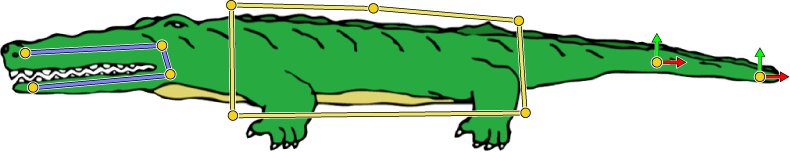
\includegraphics[scale=0.25]{alligator-avant}
  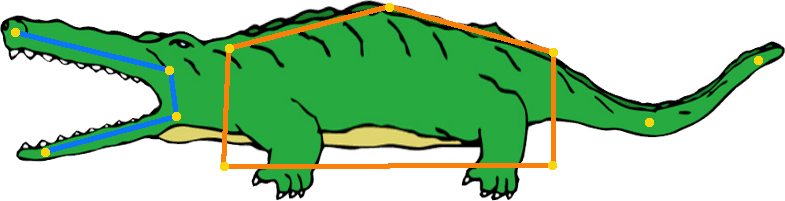
\includegraphics[scale=0.25]{alligator-apres}
  \caption{A gauche l'objet d'origine et à droite le même objet après
    déplacement de certains points de contrôle}
  \label{INTall}
\end{figure}

La finesse d'une déformation est dépendante du nombre de degrés de
liberté de l'outil, mais de même, la complexité en temps de calcul de
l'association de l'outil à l'objet en est aussi dépendante. Partant de
ce principe là, il serait intéressant de disposer de plusieurs niveaux
de résolutions d'un même outil, afin de pouvoir choisir le niveau de
résolution le plus adapté à la déformation à appliquer. Mais cela
implique la mise en place d'un moyen de communication entre les
différents niveaux de résolution, comme le modèle proposé par
\cite{Hur12} concernant les déformation de cages hiérarchiques.
\\

Tout au long de ce travail, nos contraintes sont de fournir un outil
permettant de déformer des points de l'espace de manière interactive
et fluide, ainsi que d'obtenir des formulations mathématiques simples
et claires.
%%% ----------------------------------------------------------------------


%%% Local Variables: 
%%% mode: latex
%%% LaTeX-command: "latex -shell-escape"
%%% TeX-master: "../thesis"
%%% End: 
